\section{Methodology: Global Namespace, Subtree Consistency/Durability}
\label{sec:methodology-decoupled-namespaces}

\begin{figure}[tb]
\centering
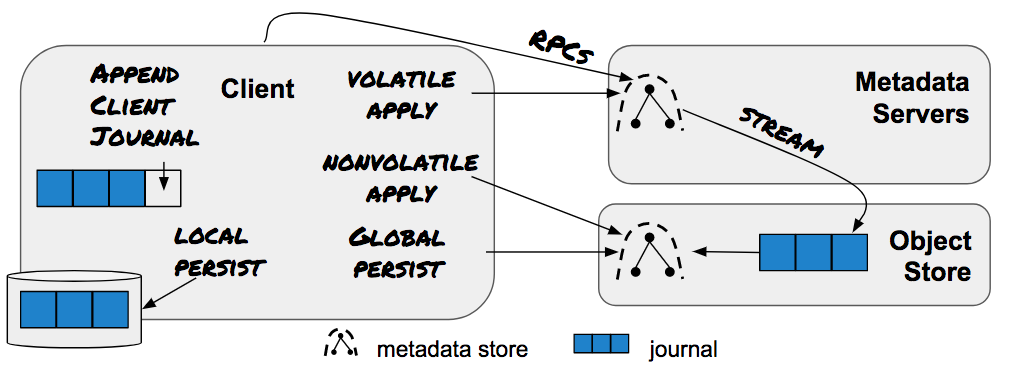
\includegraphics[width=90mm]{figures/fig-decouple.png}
\caption{Illustration of the \textbf{mechanisms} used by applications to build
consistency/durability semantics. Descriptions are provided in
Table~\ref{table:mechanisms} and the underlined words in
Section~\S\ref{sec:the-cudelesfs-mechanisms}.}\label{fig:decouple}
\end{figure}

\begin{table}
\begin{tabular}{ r | l }
  Mechanism         & Description \\\hline
  RPCs              & round trip remote procedure calls \\
  Stream            & stream journal into object store \\
  Append Client Journal & events appended to in-memory journal \\
  Volatile Apply & apply to metadata store in memory \\
  Nonvolatile Apply    & apply to metadata store in obj store \\
  Local Persist     & journal saved to client's disk \\
  Global Persist    & journal saved in object store \\
\end{tabular}
\caption{Descriptions of the mechanisms. Example compositions are shown in Table~\ref{table:spectrum}.\label{table:mechanisms}} 
\end{table}

In this section we describe Cudele, our API and framework that lets users
assign consistency and durability semantics to subtrees in the global
namespace. A \textbf{mechanism} is an abstraction and basic building block for
constructing consistency and durability guarantees. Cudele exposes these
mechanisms and the user composes them together to construct \textbf{policies}.
These policies are assigned to subtrees and they dictate how the file system
should handle operations within that subtree.  Below, we describe the
mechanisms (which are \underline{underlined}), the policies, and the API for assigning
policies to subtrees.

\subsection{Mechanisms: Building Guarantees}
\label{sec:the-cudelesfs-mechanisms}

% describe the figure
Figure~\ref{fig:decouple} shows the mechanisms (labeled arrows) in Cudele and
which daemon(s) they are performed by.  Table~\ref{table:mechanisms} has a
description of what each mechanism does.  Decoupled clients use the
\underline{Append Client Journal} mechanism to append metadata updates to a
local, in-memory journal. This is fast because clients do not need to check for
consistency when writing events and the metadata server blindly applies the
updates because it assumes the events were already checked for consistency. The
trade-off here is performance; it is a dangerous approach but could be
implemented safely if the clients or metadata server are configured to check
the validity of events before writing them.  Once the job is complete, the
system calls Cudele mechanisms to achieve the desired consistency/durability
semantics.  Cudele provides a library for clients to link into and all
operations are performed by the client.  

\subsubsection{Mechanisms Used for Consistency} \underline{RPCs} send remote procedure
calls for every metadata operation from the client to the metadata server,
assuming the request cannot be satisfied by the inode cache. This mechanism is
part of the default CephFS implementation and is the strongest form of
consistency because clients see metadata updates right away.  \underline{Nonvolatile
Apply} replays the client's journal onto the metadata cluster's metadata store.
The client's in-memory journal is written into the object store and the
metadata servers are restarted. When the metadata servers re-initialize, they
notice new journal updates in the object store and replay the events onto their
in-memory metadata stores.  \underline{Volatile Apply} takes the client's in-memory journal on the
client and applies the updates directly to the in-memory metadata store maintained
by the metadata servers. We say volatile because -- in exchange for peak
performance -- Cudele makes no consistency or durability guarantees while
Volatile Apply is executing.  If a concurrent update from a client occurs
there is no rule for resolving conflicts and if the client or metadata server
crashes there may be no way to recover.

% difference between apply and volatile apply
The biggest difference between Volatile Apply and Nonvolatile Apply is
the medium they use to communicate. Volatile Apply applies updates directly
to the metadata servers' metadata store while Nonvolatile Apply uses the
object store to communicate the journal of updates from the client to the
metadata servers.  Nonvolatile Apply is safer but has a large performance
overhead because objects in the metadata store need to be read from and written
back to the object store.

%The metadata store and journal
%are different ways of representing the namespace.  Cudele presents 6
%mechanisms: RPCs, Stream, Create, Volatile Apply, Local Persist, and Global
%Persist. ``RPCs" does round trip remote procedure calls to establish
%consistency; it is the default implementation for complying with POSIX IO in
%CephFS. ``Stream" has the metadata servers stream a journal of metadata updates
%into the object store. ``Append Client Journal" allows clients to append metadata events to an
%in-memory journal. ``Volatile apply" 
% ``Local Persist" takes the in-memory journal and writes it to the
%client's disk. ``Global Persist" saves the journal as a an object in the object
%store from the client.  Next, we discuss how these mechanisms can be composed
%to get different consistency and durability semantics. 

\subsubsection{Mechanisms Used for Durability} \underline{Stream} is one of the
mechanisms used by default in CephFS.  Using existing configuration settings in
Ceph we can turn Stream on and off.  If it is off, then the metadata servers
will not save journals in the object store. For \underline{Local Persist}, clients write
serialized log events to a file on local disk and for \underline{Global Persist},
clients push the journal into the objects store. The overheads for both Local
Persist and Global Persist is the write bandwidth of the local disk and
object store, respectively.  These persist mechanisms are part of the library that
links into the client.

\subsection{Defining Policies in Cudele}
\label{sec:setting-policies-with-cudele}

\begin{table}[t]
\begin{center}
\begin{tabular}{ l | l | l | l }
  C \(\rightarrow\) &&& \\  
  D \(\downarrow\)  	     & invisible         & weak        & strong  \\\hline
  none                       & append client journal            & append client journal          & RPCs    \\
                             &                   & +volatile apply &         \\\hdashline
  local                      & append client journal            & append client journal          & RPCs    \\
                             & +local persist    & +local persist  & +local  \\
                             &                   & +volatile apply &  persist\\\hdashline
  global                     & append client journal            & append client journal          & RPCs    \\
                             & +global persist   & +global persist & +stream \\
                             &                   & +volatile apply &         \\
\end{tabular}

\caption{Users can explore the consistency (C) and
durability (D) spectrum by composing Cudele mechanisms. 
\label{table:spectrum}}
\end{center}
\end{table}

% describe table
The spectrum of consistency and durability guarantees that users can construct
is shown in Table~\ref{table:spectrum}. The columns are the different
consistency semantics and the rows cover the spectrum of durability guarantees.
For consistency: ``invisible" means the system does not handle merging updates
into a global namespace and it is assumed that middleware or the application
manages consistency lazily; ``weak" merges updates at some time in the future
({\it e.g.}, when the system has time, when the number of updates reaches a
certain threshold, when the client is done writing, etc.); and updates in
``strong" consistency are seen immediately by all clients. For durability,
``none" means that updates are volatile and will be lost on a failure. Stronger
guarantees are made with ``local", which means updates will be retained if the
client node recovers and reads the updates from local storage, and ``global",
where all updates are always recoverable.

% which system they represent and which are impossible
Existing, state-of-the-art systems in HPC can be represented by the cells in
Table~\ref{table:spectrum} (we construct the semantics for these systems later
in Section~\S\ref{sec:microbenchmarks}).  POSIX IO-compliant systems like
CephFS and IndexFS have global consistency and durability~\footnote{This is the
normal case.  IndexFS also has bulk merge which would transition the system
into ``weak consistency"}; DeltaFS uses ``invisible" consistency and ``local"
durability and BatchFS uses ``weak" consistency and ``local" durability. These
systems have other features that could push them into different semantics but
we assign labels here based on the points emphasized in the papers.  To compose
the mechanisms users inject which mechanisms to run and which to use in
parallel using a domain specific language.  Although we can achieve all
permutations of the different guarantees in Table~\ref{table:spectrum}, not all
of them make sense. For example, it makes little sense to do \texttt{append
client journal+RPCs} since both mechanisms do the same thing or
\texttt{stream+local persist} since ``global" durability is stronger and has more
overhead than ``local" durability. The cost of each mechanism and the semantics
described above are quantified in Sections~\S\ref{sec:microbenchmarks}
and~\S\ref{sec:use-case-1}.

% talk of eventual consistency
The consistency and durability properties in Table~\ref{table:spectrum} are not
guaranteed until all mechanisms in the cell are complete. The compositions
should be considered atomic and there are no guarantees while transitioning
between policies. For example, updates are not deemed to have ``global"
durability until they are safely saved in the object store. If a failure occurs
during Global Persist or if we inject a new policy that changes a subtree from
Local Persist to Global Persist, Cudele makes no guarantee until the mechanisms
are complete. Despite this, production systems that use Cudele should state
up-front what the transition guarantees are for subtrees.

\subsection{Cudele Namespace API}
\label{sec:cudelefs-namespace-api}

% the interface
Users control consistency and durability for subtrees by contacting a daemon in
the system called a monitor, which manages cluster state changes.  Users
present a directory path and a policies configuration that gets distributed and
versioned by the monitor to all daemons in the system. For example,
(msevilla/mydir, policies.yml) would decouple the path ``msevilla/mydir" and
would apply the policies in ``policies.yml".  The policies file supports the
following parameters (default values are in parenthesis):

\begin{itemize}

  \item \texttt{consistency}: which consistency model to use (\texttt{RPCs})

  \item \texttt{durability}: which durability model to use (\texttt{stream})

  \item \texttt{allocated\_inodes}: the number of inodes to provision to the
  decoupled namespace (100)

  \item \texttt{interfere\_policy}: how to handle a request from another
  client targeted at this subtree (\texttt{allow}))

\end{itemize}

The ``Consistency" and ``Durability" parameters are set to the Cudele
mechanisms; they can be composed (\(+\)) or run in parallel (\(|\|\)).
``Allocated Inodes" is a way for the application to specify how many files it
intends to create. It is a contract so that the file system can provision
enough resources for the incumbent merge and so it can give valid inodes to
other clients. The inodes can be used anywhere within the decoupled namespace
({i.e.} at any depth in the subtree).

% description
``Interfere Policy" has two settings: \texttt{block} and \texttt{allow}.
For \texttt{block}, any requests to this part of the namespace returns with
``Device is busy", which will spare the metadata server from wasting resources
for updates that may get overwritten. If the application does not mind losing
updates, for example it wants approximations for results that take too long to
compute, it can select \texttt{allow}. In this case, metadata from the interfering client will be
written and the computation from the decoupled namespace will take priority at
merge time because the results are more accurate.

% examples
Given these default values decoupling the namespace with an empty policies file
would give the application 100 inodes but the subtree would behave like the
existing CephFS implementation.  BatchFS merges updates into the global
namespace after the job is complete.  This can be achieved with by composing
two mechanisms: 
